\chapter{Simulation par $\mathbb{P}_{1}$-interpolation}
\label{P1Interpol}
Supposons pouvoir simuler un champ gaussien $X$
sur les n\oe uds d'un maillage $M$ décrivant la fermeture d'un ouvert borné $D$.
Par une interpolation $\mathbb{P}_1$, il est possible à partir de toutes les réalisations du processus
$X$ connu en les n\oe uds de $M$, d'obtenir un nouveau processus $\tilde{X}$
sur $\bar{D}$. On aimerait que le processus $\tilde{X}$ devienne une bonne
approximation du processus $X$ (pour un maillage $M$ suffisamment raffiné)
en les n\oe uds d'un nouveau maillage $M'$ inclus dans $\bar{D}$.\\

L'intérêt pratique de la $\mathbb{P}_{1}$-interpolation est que certaines méthodes de simulation
sont très efficaces sur des maillages $M$ comme les maillages
semblables à ceux de la méthode spectrale du chapitre précédent ou
comme les maillages ne présentant pas une concentration de n\oe uds
(efficacité de la compression en $\mathcal{H}$-matrice). D'où l'idée
de transférer par $\mathbb{P}_{1}$-interpolation sur
le maillage d'intérêt $M'$, les résultats d'une simulation efficace
sur $M$.\\

\section{Cadre théorique}
\label{theory}
\noindent Soit $(\Omega,\mathcal{F},\mathbb{P})$ un espace probabilisé \\
Soit $n,d$ deux entiers naturels non nuls et $D$ un ouvert borné de $\mathbb{R}^n$  \\
On note $\lambda^n$ la mesure de Lebesgue sur $D$\\
On admet aussi que $D$ peut être décrit par un maillage triangulaire.

%Soit $X=(X_t)_{t\in \mathbb{R}^n}$ un processus gaussien centré d'ordre 2 à valeurs dans $\mathbb{R}^d$ \\
%Notons $C: \mathbb{R}^n \times \mathbb{R}^n \rightarrow M_d(\mathbb{R}) $ la fonction de covariance de $X$ \\
%Soit $M$ une triangulation de $D$ et on note $(n_i)_{i \in \{1,m\}}$ les n\oe uds
%du maillage $M$.


\begin{definition}
\label{RFmesurable}On dit que le champ aléatoire $X : D \times \Omega \rightarrow \mathbb{R}^d$ est un
champ aléatoire mesurable si $X$ est une fonction mesurable, où $D \times \Omega$
a été muni de la tribu issue de la complétion de la mesure-produit $\lambda^n \otimes \mathbb{P}$ 
\end{definition}

En se référant à \cite{ScheuererMichael2010Rots}, on obtient que tout champ aléatoire $X$ d'ordre 2 dont
les éléments diagonaux de la fonction de covariance sont des fonctions continues
admet une version $Y$ qui est mesurable. Par conséquent, pour qu'un champ
gaussien puisse être considéré comme un champ aléatoire mesurable, il suffit de
supposer que les éléments diagonaux de sa fonction de covariance soient des
fonctions continues.
~\\

Pour étudier les champs aléatoires mesurables, on introduit également l'espace de Hilbert
$(L^2_{\mathbb{R}^d}(D \times \Omega, \lambda^n \otimes \mathbb{P}),\|\cdot\|)$,  l'ensemble des fonctions $\phi$ de $D \times \Omega$ dans
$\mathbb{R}^d$ telles que:
~\\
\begin{itemize}
\item $\phi$ est $(\mathcal{B}(D) \otimes \mathcal{F},\mathcal{B}(\mathbb{R}^d))$-mesurable
\item la quantité
$\|\phi\|^2 = \mathbb{E}(\displaystyle\int_D \|\phi(t,.)\|_2^2 \ud \lambda^n(t))$ est finie
\end{itemize}
~\\
\noindent Ainsi, un champ aléatoire mesurable $X$ est dans
$L^2_{\mathbb{R}^d}(D \times \Omega , \lambda^n \otimes \mathbb{P}) $ si et seulement si $\|X\|$ est une quantité finie.


\section{Approximation d'une fonction par méthode des éléments finis $\mathbb{P}_1$}

L'approximation $\mathbb{P}_1$-Lagrange est une manière très classique en analyse numérique d'approcher la
solution d'une EDP (équation aux dérivées partielles). Par conséquent, tout lecteur qui souhaitera des détails
sur ce procédé pourra se référer au livre de Grégoire Allaire \cite{alma991003727179806616}. De ce livre, on utilise
notamment les définitions de maillage triangulaire ou triangulation (page 175) et de suite de maillages réguliers (page 188).\\
~\\
Rappelons rapidement en quoi consiste l'approximation d'une fonction par la méthode des éléments finis.
On considère un maillage triangulaire $M$ décrivant la fermeture de $D$ ($D$ peut être supposé connexe). Si on note $(n_i)_{i \in \llbracket 1,m \rrbracket}$  les n\oe uds de $M$, on dispose
d'un unique $m$-uplet $(\psi_1, \cdots, \psi_m)$ de fonctions continues de $\bar{D}$ dans $\mathbb{R}$ et polynomiales de degre $1$ sur
chaque $n$-simplexe du maillage $M$ et tel que:
\begin{equation*}
  \forall (i,j) \in \llbracket 1,m \rrbracket^2, \psi_i(n_j) = \delta_{i,j}
\end{equation*}

\begin{remark}
On appelle les $\psi_i$, les fonctions de base du maillage $M$ 
\end{remark}

On définit alors pour $f: \bar{D} \rightarrow \mathbb{R}^d$ une fonction continue sur $D$, $R_{M,d}(f)$, l'interpolée $\mathbb{P}_1$ de $f$
comme la fonction telle que:
\begin{equation}
  \label{ContiInterpol}
  \forall t \in \bar{D}, \; R_{M,d}(f)(t) = \displaystyle\sum_{i=1}^m \psi_i (t)\cdot f(n_i)
\end{equation}

\begin{remark}
  $R_{M,d}(f)$ prend les mêmes valeurs que $f$ en les n\oe uds du maillage
\end{remark}
~\\
L'opérateur d'interpolation $R_{M,d}$ décrit l'approximation par interpolation $\mathbb{P}_1$-Lagrange des fonctions continues sur $\bar{D}$.
Dans le livre de Grégoire Allaire, tout est présenté dans le cas où $d = 1$, notamment les espaces de Sobolev qui seront utiles
pour faire des estimations. Cependant, il n'est guère difficile de généraliser la définition des espaces de Sobolev dans le cas $d > 1$ comme il va suivre.

\section{Espaces de Sobolev et interpolation}

On suppose que le lecteur est familier avec les espaces de Sobolev
notés $W^{k,p}(O)$ ou $H^{k}(O)$, où $O$ est un ouvert. On peut ainsi présenter une légère généralisation des espaces de Sobolev où
les (classes de) fonctions sont à valeurs dans $\mathbb{R}^d$, où $d$ est
éventuellement strictement supérieur à 1.

\begin{definition}
Pour $O$ un ouvert de $\mathbb{R}^n$, pour $k \in \mathbb{N}^{*}$ et $p \in [1,\infty]$:
\begin{equation*}
  W^{k,p}_{\mathbb{R}^d}(O) = \{ f = (f_1, \cdots, f_d)^{T}: O \rightarrow \mathbb{R}^d \; /\; \forall i \in \llbracket 1,d \rrbracket, \; f_i \in W^{k,p}(O) \}\\
\end{equation*}
\end{definition}
\noindent On se servira par la suite surtout de cet ensemble:
\begin{equation*}
  H^{k}_{\mathbb{R}^d}(O) = W^{k,2}_{\mathbb{R}^d}(O)
\end{equation*}

\begin{property}
  Pour $k \in \mathbb{N}^{*}$, l'espace $H^{k}_{\mathbb{R}^d}(O)$ est un espace de
  Hilbert s'il est muni de la norme
  \smash{\mbox{$\|\cdot \|_{H^{k}_{\mathbb{R}^d}(O)}$}} telle que pour
  $f \in H^{k}_{\mathbb{R}^d}(O)$:
  \begin{equation*} \|f\|_{H^{k}_{\mathbb{R}^d}(O)}^2 = \displaystyle\sum_{i = 1}^d \|f_i\|_{H^{k}(O)}^2  \end{equation*}
\end{property}
~\\
Avec ces définitions, notons les 2 propriétés suivantes:

\begin{property}
Pour tout maillage triangulaire $M$ de $\bar{D}$ et toute fonction continue $f: \bar{D} \rightarrow \mathbb{R}^d, \;R_{M,d}(f) \in H^{1}_{\mathbb{R}^d}(D)$
\end{property}

\begin{property}[Injection de Sobolev]
Soit $k \in \mathbb{N}$ tel que $k+1 > n/2$.\\$\forall w \in H^{k+1}_{\mathbb{R}^d}(D)$, $w$ est la restriction sur $D$ d'une fonction continue sur $\bar{D}$.
\end{property}

On est maintenant apte à introduire un théorème majeur pour la suite ainsi que son corollaire. Considérons $(\mathcal{T}_h)_{h \in \mathbb{R}^{*}_{+}}$ une suite de maillages (triangulaires) réguliers de $\bar{D}$. On rappelle que le paramètre $h$ désigne le maximum des diamètres des $n$-simplexes qui composent le maillage $\mathcal{T}_h$.
Pour $h \in \mathbb{R}^{*}_{+}$, on note $R_{h,d}$ l'opérateur d'interpolation $R_{\mathcal{T}_h,d}$. 

\begin{theorem}
  Soit $k \in \mathbb{N}$ tel que $k+1 > n/2$. Il existe $C \in \mathbb{R}^{*}_{+}$ tel que:
  \begin{equation*}
    \forall h \in  \mathbb{R}^{*}_{+}, \forall v \in H^{k+1}(D), \;
    \|v - R_{h,1}(v) \|_{H^{1}(D)} \leq C h^k \|v\|_{H^{k+1}(D)}
  \end{equation*}
\end{theorem}

\begin{corollary}
  \label{ineqInterpol}
  Soit $k \in \mathbb{N}$ tel que $k+1 > n/2$. Il existe $C \in \mathbb{R}^{*}_{+}$ tel que:
  \begin{equation*}
    \forall h \in  \mathbb{R}^{*}_{+}, \forall v \in H^{k+1}_{\mathbb{R}^d}(D), \;
    \|v - R_{h,d}(v) \|_{H^{1}_{\mathbb{R}^d}(D)} \leq C h^k \|v\|_{H^{k+1}_{\mathbb{R}^d}(D)}
  \end{equation*}
\end{corollary}


\section{Espaces de Sobolev et champs aléatoires}

Lorsque l'on étudie les réalisations d'un champ aléatoire, on peut s'interroger
sur la régularité des trajectoires (continuité, différentiabilité). Dans cette
section, on exhibe des conditions pour qu'un champ aléatoire mesurable (voir
la définition~\ref{RFmesurable}) puisse admettre presque sûrement que des
trajectoires dans un espace de Sobolev. Tout ce qui suit est fondé en grande partie sur
le livre de Hristopulos \cite{alma991004158221006616}, l'article de Scheuerer \cite{ScheuererMichael2010Rots} et le chapitre 4 de \textit{``The Theory of Stochastic Processes I''}~\cite{GihmanSkoro}. 


\subsection{Sur la différentiabilité en moyenne quadratique d'un champ aléatoire}

\`A la page 183 dans \cite{alma991004158221006616}, pour $X: D \times \Omega \rightarrow \mathbb{R}$
un champ aléatoire d'ordre 2 et $i \in \llbracket 1;n \rrbracket$, on définit, si elle existe,
la dérivée partielle de $X$ en moyenne
quadratique par rapport à la $i$\up{ème} variable que l'on note $\frac{\partial}{\partial x_i} X$ ou $\frac{\partial X}{\partial x_i}$. On remarque que sa définition ne
revient qu'à dire que l'application $\gamma: D \rightarrow L^2(\Omega,\mathbb{P})$
qui à $t \in D$ associe $\gamma(t) = X(t,.)$ admet une dérivée
partielle par rapport à la $i$\up{ème} variable sur $D$.\\
~\\
On peut alors définir, si elles existent, les dérivées partielles en moyenne quadratique sur $D$ d'ordre supérieur à 1 de
$X$, $\frac{\partial^{k}}{\partial x_{\alpha_1} \cdots \partial x_{\alpha_k} } X$ où $\alpha_1, \cdots , \alpha_k$ sont $k$ entiers entre $1$ et $n$ et où la notation indique qu'on a dérivé par rapport à
la $\alpha_k$\up{ème} variable (en moyenne quadratique) , puis par rapport à la $\alpha_{k-1}$\up{ème} variable, ainsi de suite et à la fin par rapport à la $\alpha_{1}$\up{ème} variable. On dira alors que $\frac{\partial^{k}}{\partial x_{\alpha_1} \cdots \partial x_{\alpha_k} } X$  est une dérivée partielle (en moyenne quadratique) de $X$ d'ordre $k$.

~\\On s'apprête à mettre en avant une condition suffisante pour qu'un champ aléatoire d'ordre 2 et centré admette des dérivées partielles en moyenne quadratique. Mais il
faut d'abord introduire le concept de dérivée généralisée mixte. Considérons \mbox{$X: D \times \Omega \rightarrow \mathbb{R}$} un champ
aléatoire d'ordre 2, centré et dont on note la fonction de covariance
$C: D \times D \rightarrow \mathbb{R}$

\begin{definition}
  Soit $i \in \llbracket 1;n \rrbracket$ et $(s,t) \in D \times D $. On note $e_i$ le
  $i$\up{ème} vecteur de la base canonique de $\mathbb{R}^n$.\\

  On dit alors que $C$ admet une dérivée mixte généralisée en $(s,t)$ par
  rapport à la $i$\up{ème} variable si
  \begin{equation}
    \lim_{(h,k) \to (0,0)} \frac{C(s+h\cdot e_i\;,\;t+k\cdot e_i)-C(s,\;t+k\cdot e_i)-C(s+h\cdot e_i \;,t)+C(s,t)}{hk}
  \end{equation}
  existe. Si tel est le cas, on notera cette limite $(D^{i,i}C)(s,t)$.\\
\end{definition}

\begin{remark}
  On peut voir $D^{i,i}$ comme un opérateur ayant pour ensemble de départ et d'arrivée l'ensemble des fonctions allant de $D \times D$ dans $\mathbb{R}$
\end{remark}

\begin{theorem}
  Pour $i \in \llbracket 1;n \rrbracket$, $X$ admet une dérivée partielle en moyenne quadratique par rapport
  à la $i$\up{ème} variable si et seulement $\forall t \in D$, $(D^{i,i}C)(t,t)$ existe et est fini. \\

  \noindent Si tel est le cas, alors $\forall (s,t) \in D \times D$, $(D^{i,i}C)(s,t)$ existe et est finie. De plus:
  \begin{equation} \mathbb{E}\biggl(\frac{\partial X}{\partial x_i} (s) \frac{\partial X}{\partial x_i} (t)\biggl) = (D^{i,i}C)(s,t) \end{equation}
\end{theorem}

\begin{remark}
  Ce théorème explicite donc la fonction de covariance de $\frac{\partial X}{\partial x_i}$.
\end{remark}

\begin{definition}
\noindent Soit $\alpha_1, \cdots , \alpha_k$ $k$ entiers entre $1$ et $n$.\\
\begin{itemize}  
\item On définit $D^{(\alpha_1, \alpha_1), \cdots, (\alpha_k, \alpha_k)}$ comme l'opérateur $D^{\alpha_1, \alpha_1} \circ \cdots \circ D^{\alpha_k, \alpha_k}$.\\

\item Soit $\kappa \in \mathbb{N}^n$ tel que $\forall i \in \llbracket 1;n \rrbracket$, $\kappa_i$ indique
  le nombre d'éléments parmi les $k$ entiers $\alpha_1, \cdots , \alpha_k$ qui prennent la valeur $i$.\\
  
\noindent Alors si pour tout permutation de $\llbracket 1;k \rrbracket$, $D^{(\alpha_{\sigma(1)}, \alpha_{\sigma(1)}), \cdots, (\alpha_{\sigma(k)}, \alpha_{\sigma(k)})}C$
  est bien défini sur $D \times D$ et que $D^{(\alpha_{\sigma(1)}, \alpha_{\sigma(1)}), \cdots, (\alpha_{\sigma(k)}, \alpha_{\sigma(k)})}C = \\D^{(\alpha_1, \alpha_1), \cdots, (\alpha_k, \alpha_k)}C$,
  alors on définit $D^{\kappa}C$ comme étant la fonction \\$D^{(\alpha_1, \alpha_1), \cdots, (\alpha_k, \alpha_k)}C$.
\end{itemize}
\end{definition}


\begin{corollary}
Soit $\alpha_1, \cdots , \alpha_k$ $k$ entiers entre $1$ et $n$, $(s,t) \in D \times D $.\\
\noindent La dérivée partielle en moyenne quadratique $\frac{\partial^{k}}{\partial x_{\alpha_1} \cdots \partial x_{\alpha_k} } X$ existe si et seulement si $\forall t \in D$, la quantité $(D^{(\alpha_1, \alpha_1), \cdots, (\alpha_k, \alpha_k)}C)(t,t)$ est bien définie et finie.\\

\noindent Si tel est le cas, alors $\forall (s,t) \in D \times D$, $(D^{(\alpha_1, \alpha_1), \cdots, (\alpha_k, \alpha_k)}C)(s,t)$ est défini et fini. De plus:
  \begin{equation} \mathbb{E}\biggl(\frac{\partial^{k}X}{\partial x_{\alpha_1} \cdots \partial x_{\alpha_n} } (s) \frac{\partial^{k}X}{\partial x_{\alpha_1} \cdots \partial x_{\alpha_n} }(t)\biggl) = (D^{(\alpha_1, \alpha_1), \cdots, (\alpha_k, \alpha_k)}C)(s,t) \end{equation}
\end{corollary}
~\\
\begin{property}
Soit $(s,t) \in D \times D $ et $m \in \mathbb{N}$.\\
\noindent Si $C$ est une fonction de classe $\mathcal{C}^{2m}$ sur $D \times D$ alors $\forall \kappa \in \mathbb{N}^d$ tel que $|\kappa| \leq m$,
$D^{\kappa}C$ est bien définie sur $D \times D$ et $\forall (s,t) \in D \times D$:
\begin{equation}
  (D^{\kappa}C)(s,t)= \frac{\partial^{2|\kappa|}}{\partial s_1^{\kappa_1} \cdots \partial s_n^{\kappa_n} \partial t_1^{\kappa_1} \cdots \partial t_n^{\kappa_n}} (s,t)
\end{equation}
\end{property}

\subsection{Résultat de régularité des trajectoires}

On dédie cette sous-section à un autre résultat important qui permet de déduire une estimation théorique en lien avec la simulation d'un processus gaussien par méthode de $\mathbb{P}_1$-interpolation présentée à la section suivante. Ce résultat est tiré de l'article de Scheuerer \cite{ScheuererMichael2010Rots}. \`A partir de la preuve
évoquée dans l'article, il est possible de raffiner un peu plus le propos, ce
qui s'avèrera nécessaire pour justifier des propriétés mathématiques de la future méthode.

\begin{theorem}
  Soit $O$ un ouvert de $\mathbb{R}^n$, $X: O \times \Omega \rightarrow \mathbb{R}$ un champ aléatoire
  mesurable dont on note $C: O \times O \rightarrow \mathbb{R}$ la fonction
  de covariance. Soit $k \in \mathbb{N}^{*}$.\\
\noindent Alors si pour tout
  $\alpha \in \mathbb{N}^{n}$ tel que $|\alpha| \leq k$, $D^{\alpha}C$ existe
  sur $O \times O$ et est continue sur la diagonale de $O \times O$, alors
  les trajectoires de $X$ sont presque sûrement dans $H_{loc}^{k}(O)$ et pour
  tout $\alpha \in \mathbb{N}^{n}$ tel que $|\alpha| \leq k$, $\mathbb{P}(\omega)-$presque sûrement, la dérivée en moyenne quadratique $\frac{\partial^{|\alpha|}}{\partial x_{1}^{\alpha_1} \cdots \partial x_{n}^{\alpha_n} } X(.,\omega)$ coincide presque partout (pour la mesure de Lebesgue dans $O$) avec la dérivée faible d'indice $\alpha$ de $X(.,\omega), \; \partial^{\alpha} X(.,\omega)$.\\
~\\  
  Si de plus pour tout $\alpha \in \mathbb{N}^{n}$ tel que $|\alpha| \leq k$:
  \begin{equation}
  \displaystyle\int_O D^{\alpha}C(t,t) dt < +\infty
  \end{equation}

\noindent Alors on a même que les trajectoires de $X$ sont presque sûrement dans $H^{k}(O)$ (ce qui revient à dire que pour tout $\alpha \in \mathbb{N}^{n}$,
  $\mathbb{P}(\omega)-$presque sûrement $\partial^{\alpha} X(.,\omega)$ est dans $L^2(O)$).
\end{theorem}

\begin{corollary}
  \label{RFcorollary}
Soit $O$ un ouvert de $\mathbb{R}^n$, $X = (X_1, \cdots, X_d): O \times \Omega \rightarrow \mathbb{R}^d$ un champ aléatoire
  mesurable dont on note $C = (C_{i,j}): O \times O \rightarrow M_d(\mathbb{R})$ la fonction
  de covariance. Soit $k \in \mathbb{N}^{*}$.\\
\noindent Si pour tout $i \in \llbracket 1;d \rrbracket$,
  $\alpha \in \mathbb{N}^{n}$ tel que $|\alpha| \leq k$, $D^{\alpha}C_{i,i}$ existe
sur $O \times O$, est continue sur la diagonale de $O \times O$, et que
\begin{equation}
\displaystyle\int_O D^{\alpha}C_{i,i}(t,t) dt < +\infty
\end{equation}
alors
  les trajectoires de $X$ sont presque sûrement dans $H_{\mathbb{R}^d}^{k}(O)$ et pour \\$i \in \llbracket 1;d \rrbracket$ et $\alpha \in \mathbb{N}^{n}$ tel que $|\alpha| \leq k$, $\mathbb{P}(\omega)-$presque sûrement, la dérivée en moyenne quadratique $\frac{\partial^{|\alpha|}}{\partial x_{1}^{\alpha_1} \cdots \partial x_{n}^{\alpha_n} } X_i(.,\omega)$ coincide dans $L^2(O)$ avec la dérivée faible d'indice $\alpha$ de $X_i(.,\omega), \; \partial^{\alpha} X_i(.,\omega)$.
\end{corollary}

Avec ce théorème, nous avons tous les outils nécessaires pour justifier les
propriétés théoriques de la méthode de simulation par $\mathbb{P}_1$-interpolation.

\section{Méthode de $\mathbb{P}_1$-interpolation}

\subsection{Description de la méthode}

Considérons $X: \bar{D} \times \Omega \rightarrow \mathbb{R}^d$ un champ
aléatoire mesurable gaussien centré dont on note
$C: \bar{D} \times \bar{D} \rightarrow M_d(\mathbb{R})$ la fonction de
covariance. Soit $M$ un maillage triangulaire de $\bar{D}$ dont on note $(n_i)_{i \in \llbracket 1;m \rrbracket}$ les $m$ n\oe uds du maillage $M$. On note $(\psi_i)_{i \in \llbracket 1;m \rrbracket}$ les fonctions de base du maillage $M$.\\

\noindent On définit alors l'interpolée $\mathbb{P}_1$ de $X$ (par le maillage $M$), le processus
$\mathcal{R}_{M,d}X$ définit de la fonction suivante: 

\begin{equation}
  \label{RFInterpol}
  \forall (t,\omega) \in \bar{D} \times \Omega, \; (\mathcal{R}_{M,d}X)(t,\omega) =  \displaystyle\sum_{i=1}^m \psi_i (t)\cdot X(n_i,\omega)
\end{equation}

\noindent On appellera l'opérateur $\mathcal{R}_{M,d}$, l'opérateur d'interpolation $\mathbb{P}_1$ (qu'on applique ici à des champs aléatoires à valeurs dans $\mathbb{R}^d$).
\begin{remark}
Comme $X$ est un champ gaussien, il s'avère que $\mathcal{R}_{M,d}X$ est aussi un champ gaussien.
\end{remark}

\` A partir de ce nouveau processus, si on dispose de $M'$ un maillage qui décrit la fermeture d'un ouvert inclus dans $D$, on désire étudier le
processus $\mathcal{R}_{M,d}X$ en les n\oe uds du maillage $M'$ en se demandant s'il
approche bien le processus $X$ en les points du maillage $M'$. La prochaine sous-section donne un début d'élément de réponse en exhibant
une forme de convergence mais cette convergence ne dit aucunement qu'en raffinant le maillage $M$ alors l'interpolée converge en loi en
les n\oe uds du maillage $M'$ vers le processus $X$.\\

Par ailleurs, une telle méthode suppose que l'on sait simuler $X$ en les n\oe uds de $M$. Donc la complexité en temps et en mémoire
de l'algorithme associé à la méthode dépend du choix de simulation de $X$ en les n\oe uds de $M$. Néanmoins une fois qu'on connaît
en les n\oe uds $(n_i)_{i \in \llbracket 1;m \rrbracket}$ les valeurs $X(n_i,\omega)$, la $\mathbb{P}_1$-interpolation qui donne
en les n\oe uds $(\tilde{n_{i}})_{i \in \llbracket 1;\tilde{m} \rrbracket}$ de $M'$ les $(\mathcal{R}_{M,d}X)(\tilde{n_{i}},\omega)$, admet une complexité algorithmique indépendante
du choix de simulation. Sur OpenTURNS, l'implémentation des maillages de dimension $n$ allant de $1$ à $3$ à l'aide
d'une structure hiérarchique de données de type k-d tree permet d'accélérer la $\mathbb{P}_1$-interpolation. Sans entrer
dans les détails, si on suppose que $d \leq 3$ et que tous les maillages $M$ et $M'$ étudiés admettent une borne uniforme sur le
nombre de $n$-simplexes partageant un même n\oe ud, alors la complexité temporelle de la $\mathbb{P}_1$-interpolation
est en $O(\tilde{m}.log(m))$. Sous ces mêmes hypothèses, on obtient une complexité mémoire en $O(m+\tilde{m})$.


\subsection{Estimation d'erreur}

Le théorème suivant donne un cadre pertinent quant à l'utilisation de la méthode de $\mathbb{P}_1$-interpolation.
Considérons d'abord $(\mathcal{T}_h)_{h \in \mathbb{R}^{*}_{+}}$ une suite de maillages réguliers de $\bar{D}$
dont on note $\mathcal{R}_{h,d}$ leur opérateur d'interpolation $\mathbb{P}_1$
de champs aléatoires à valeurs dans $\mathbb{R}^d$ défini par la formule~(\ref{RFInterpol}) et $R_{h,d}$  leur opérateur d'interpolation $\mathbb{P}_1$ de fonctions continues de $\bar{D}$ dans $\mathbb{R}^d$ défini par la formule~(\ref{ContiInterpol}) pour le maillage $\mathcal{T}_h$.

\begin{theorem}
\label{EstimeeTheo}
Soit $k \in \mathbb{N}$ tel que $k+1 > n/2$. Si pour tout $i \in \llbracket 1;d \rrbracket$, $\alpha \in \mathbb{N}^{n}$ tel que $|\alpha| \leq k+1$, $D^{\alpha}C_{i,i}$ existe
sur $D \times D$, est continue sur la diagonale de $D \times D$, et tel que
\begin{equation}
\displaystyle\int_D D^{\alpha}C_{i,i}(t,t) dt < +\infty
\end{equation}

\noindent alors $X$ admet presque sûrement des trajectoires dans $H^{k+1}_{\mathbb{R}^d}(D)$ (donc des trajectoires continues sur $\bar{D}$) et il existe une constante $K \in \mathbb{R}_{+}$ tel que $\forall h \in \mathbb{R}_{+}^{*}$:

\begin{equation}
\|X - \mathcal{R}_{h,d}X \| \leq K \cdot h^{k} 
\end{equation}
\end{theorem}

\begin{remark}
$\| \cdot \|$ est la norme définie à la fin de la section~\ref{theory}.
\end{remark}

\begin{remark}
  Ce résultat ne nécessite pas que $X$ soit un champ gaussien. Le résultat
  reste donc valide sans cette hypothèse.
\end{remark}

\begin{proof}
  En utilisant le corollaire~\ref{RFcorollary}, on obtient que les trajectoires
  de $X$ sont presque sûrement dans $H^{k+1}_{\mathbb{R}^d}(D)$ et que $\mathbb{P}(\omega)$-presque sûrement,
  pour tout $i \in \llbracket 1;d \rrbracket$ et $\alpha \in \mathbb{N}^{n}$ tel que $|\alpha| \leq k+1$,
  $\frac{\partial^{|\alpha|}}{\partial x_{1}^{\alpha_1} \cdots \partial x_{n}^{\alpha_n} } X_i(.,\omega) = \partial^{\alpha}X_i(.,\omega)$ dans $L^2(D,\lambda^n)$.
  Donc par le corollaire~\ref{ineqInterpol}, on dispose de $L \in \mathbb{R}_{+}^{*}$ tel que,
  $\mathbb{P}(\omega)$-presque sûrement, pour tout $h \in \mathbb{R}^{*}_{+}$:
  \begin{eqnarray*}
    \|X(.,\omega) - \mathcal{R}_{h,d}(X(.,\omega)) \|_{H^{1}_{\mathbb{R}^d}(D)}^2 &=& \|X(.,\omega) - R_{h,d}(X(.,\omega)) \|_{H^{1}_{\mathbb{R}^d}(D)}^2 \\
    &\leq& L^2 \cdot h^{2k} \cdot \|X(.,\omega)\|_{H^{k+1}_{\mathbb{R}^d}(D)}^2
  \end{eqnarray*}

  \noindent De plus $\mathbb{P}(\omega)$-presque sûrement:
  \begin{eqnarray*}
    \|X(.,\omega)\|_{H^{k+1}_{\mathbb{R}^d}(D)}^2 &=& \displaystyle\sum_{i=1}^{d}  \displaystyle\sum_{\substack{\alpha \in \mathbb{N}^n \\ |\alpha| \leq k+1}} \int_D |\partial^{\alpha}X_i(t,\omega)|^2 dt \\
                                          &=& \displaystyle\sum_{i=1}^{d}  \displaystyle\sum_{\substack{\alpha \in \mathbb{N}^n \\  |\alpha| \leq k+1} } \int_D |\frac{\partial^{|\alpha|}}{\partial x_{1}^{\alpha_1} \cdots \partial x_{n}^{\alpha_n} } X_i(.,\omega)|^2 dt
  \end{eqnarray*}

  \noindent Donc par passage à l'espérance, pour tout $h \in \mathbb{R}^{*}_{+}$:
\footnotesize{
  \begin{eqnarray*}
    \mathbb{E}(\|X(.,\omega) - \mathcal{R}_{h,d}(X(.,\omega)) \|_{H^{1}_{\mathbb{R}^d}(D)}^2) &\leq& L^2 \cdot h^{2k} \cdot \displaystyle\sum_{i=1}^{d} \; \mathbb{E}(\|X(.,\omega)\|_{H^{k+1}_{\mathbb{R}^d}(D)}^2) \\
    &=& L^2 \cdot h^{2k} \cdot \displaystyle\sum_{i=1}^{d} \displaystyle\sum_{\substack{\alpha \in \mathbb{N}^n \\  |\alpha| \leq k+1} } \mathbb{E}\biggl(\int_D |\frac{\partial^{|\alpha|}}{\partial x_{1}^{\alpha_1} \cdots \partial x_{n}^{\alpha_n} } X_i(.,\omega)|^2 dt \biggl) \\
    &=& L^2 \cdot h^{2k} \cdot \displaystyle\sum_{i=1}^{d} \displaystyle\sum_{\substack{\alpha \in \mathbb{N}^n \\  |\alpha| \leq k+1} } \int_D \mathbb{E}\biggl(|\frac{\partial^{|\alpha|}}{\partial x_{1}^{\alpha_1} \cdots \partial x_{n}^{\alpha_n} } X_i(.,\omega)|^2 \biggl) dt \\
    &=& L^2 \cdot h^{2k} \cdot \displaystyle\sum_{i=1}^{d} \displaystyle\sum_{\substack{\alpha \in \mathbb{N}^n \\  |\alpha| \leq k+1} } \int_D D^{\alpha}C_{i,i}(t,t) dt \\
    &< &+\infty
  \end{eqnarray*}
}

\normalsize{
\noindent Or pour tout $h \in \mathbb{R}^{*}_{+}$:}
\footnotesize{\begin{equation*}
\|X - \mathcal{R}_{h,d}X\|^2 \leq \mathbb{E}(\|X(.,\omega) - \mathcal{R}_{h,d}(X(.,\omega)) \|_{H^{1}_{\mathbb{R}^d}(D)}^2)
\end{equation*}}

\normalsize{\noindent Donc finalement:}
\footnotesize{\begin{equation*}
\|X - \mathcal{R}_{h,d}X\| \leq \biggl(L \; \cdot \biggl(\displaystyle\sum_{i=1}^{d} \displaystyle\sum_{\substack{\alpha \in \mathbb{N}^n \\  |\alpha| \leq k+1} } \int_D D^{\alpha}C_{i,i}(t,t) dt \biggr)^{1/2} \biggr) \cdot h^k 
\end{equation*}}

\end{proof}

\begin{corollary}[Convergence en loi]
  Sous les mêmes hypothèses que le théorème~\ref{EstimeeTheo} et en supposant de plus que $k$ est un entier non nul
  alors pour toute fonction $\phi: L^2_{\mathbb{R}^d}(D,\lambda^n) \rightarrow \mathbb{R}$ continue et bornée, on a:
  \begin{equation}
   \mathbb{E}(\phi(\mathcal{R}_{h,d}X(.,\omega))) \underset{\substack{h \to 0 \\ h>0}}{\rightarrow} \mathbb{E}(\phi(X(.,\omega)))
  \end{equation}
\end{corollary}

\begin{proof}
  Soit $(u_n)_{n \in \mathbb{N}}$ une suite de réels strictement positifs tendant vers $0$ et
  $\psi: \mathbb{N} \rightarrow \mathbb{N}$ une extractrice. On a donc que $(u_{\psi(n)})_{n \in \mathbb{N}}$ tend aussi vers $0$.\\

  \noindent Par le théorème précédent et l'hypothèse que $k$ est non nul, on a que \begin{equation*}\|X - \mathcal{R}_{h,d}X\|  \underset{h \to 0}{\rightarrow} 0\end{equation*}
  donc en particulier \begin{equation*}\mathbb{E}(\|X(.,\omega) - \mathcal{R}_{u_{\psi(n)},d}X(.,\omega)\|_{L^2_{\mathbb{R}^d}(D,\lambda^n)}^2) \underset{n \to \infty}{\rightarrow} 0\end{equation*}
  Par conséquent, on dispose de $\theta: \mathbb{N} \rightarrow \mathbb{N}$ une extractrice telle que $\mathbb{P}(\omega)$-presque sûrement
  \begin{equation*}\|X(.,\omega) - \mathcal{R}_{u_{\psi(\theta(n))},d}X(.,\omega)\|_{L^2_{\mathbb{R}^d}(D,\lambda^n)}^2 \underset{n \to \infty}{\rightarrow} 0\end{equation*}
  \noindent D'où par continuité de $\phi$, $\mathbb{P}(\omega)$-presque sûrement
  \begin{equation*}\phi(\mathcal{R}_{u_{\psi(\theta(n))},d}X(.,\omega)) \underset{n \to \infty} {\to}\phi(X(.,\omega))\end{equation*} Comme $\phi$ est bornée, on peut appliquer le théorème de convergence dominée pour
  obtenir: \begin{equation*} \mathbb{E}(\phi(\mathcal{R}_{u_{ \psi(\theta(n)) },d}X(.,\omega))) \underset{n \to \infty}{\rightarrow}  \mathbb{E}(\phi(X(.,\omega))) \end{equation*}

  \noindent Finalement on vient de prouver que de toute suite extraite de $(u_n)_{n \in \mathbb{N}}$, $(u_{\phi(n)})_{n \in \mathbb{N}}$, il existe une extractrice $\theta$ telle
  que $\mathbb{E}(\phi(\mathcal{R}_{u_{\psi(\theta(n))},d}X(.,\omega))) \underset{n \to \infty}{\rightarrow}  \mathbb{E}(\phi(X(.,\omega)))$. Par conséquent la suite
  $(\mathbb{E}(\phi(\mathcal{R}_{u_n,d}X(.,\omega))))_{n \in \mathbb{N}}$ converge et
  \begin{equation*}
    \mathbb{E}(\phi(\mathcal{R}_{u_n,d}X(.,\omega))) \underset{n \to \infty}{\rightarrow}  \mathbb{E}(\phi(X(.,\omega)))
  \end{equation*}
  Comme ce résultat est vrai pour toute suite $(u_n)_{n \in \mathbb{N}}$ de réels strictement positifs tendant vers $0$, on a donc prouvé par caractérisation
  séquentielle le résultat recherché: \begin{equation*} \mathbb{E}(\phi(\mathcal{R}_{h,d}X(.,\omega))) \underset{\substack{h \to 0 \\ h>0}}{\rightarrow}  \mathbb{E}(\phi(X(.,\omega))) \end{equation*}
\end{proof}


\section{Erreur et convergence numérique}
\label{P1interpolConvErr}
%problèmes restants:
%-décrire la seconde partie de la construction du maillage d'intérêt 
%-faire un choix de tests qui valident mieux la méthode de simulation
%en variant le nombre de réalisations
La méthode de $\mathbb{P}_{1}$-interpolation nécessite la connaissance d'un ouvert $D \subset \mathbb{R}^n$, d'un maillage triangulaire
$M$ (notons $n_M$ son nombre de n\oe uds) discrétisant le domaine $\bar{D}$ et d'un maillage triangulaire d'intérêt $M'$ (notons $n_{M'}$ son nombre de n\oe uds)
dont les simplexes sont inclus dans $\bar{D}$ et d'une fonction de covariance $C: \bar{D} \times \bar{D} \rightarrow \mathbb{R}^{d}$.
Ainsi en utilisant une méthode de simulation en les n\oe uds
de $M$ du champ gaussien $X$ centré et caractérisé par $C$, on effectue une $\mathbb{P}_{1}$-interpolation à partir
d'une réalisation sur $M$, pour obtenir une réalisation de $\mathcal{R}_{M,d}X$ en les n\oe uds de $M'$.
Pour les tests, on ne considérera que $n \in \{2,3\}$ et la méthode de Cholesky sera utilisée pour simuler en les n\oe uds
de $M$.%question sur la complexité en temps et mémoire

\subsection{Dimension n=2}

On choisit $\bar{D}= [-1,1]^2$ et pour $m \in \mathbb{N}^{*}, \; m > 1$, le maillage $M$ sera caractérisé par des n\oe uds du type
\begin{equation*} \biggl (\biggl(-1 + \frac{2i}{m-1}, -1 + \frac{2j}{m-1} \biggr)\biggr)_{(i,j) \in \llbracket 0;m-1 \rrbracket^2}  \end{equation*}
et leurs éléments triangulaires sont décrits de la même façon qu'à la sous-section~\ref{choDim2} du chapitre~\ref{chapCholesky}.
Si on note $h_M$ le maximum des diamètres des éléments triangulaires qui composent le maillage $M$, $h_M = \sqrt{2} \cdot \frac{2}{m-1}$ .\\
On fera varier le nombre de n\oe uds $n_M = m^2$ entre $10$ et $10000$ et on ne considérera qu'une seule fonction de covariance $C$:
\begin{equation*} C(x,y) = \exp\biggl(-\biggl(\frac{y_1 - x_1}{b_1}\biggr)^2-\biggl(\frac{y_2 - x_2}{b_2}\biggr)^2\biggr) \end{equation*}
pour $(x,y)= ((x_1,x_2),(y_1,y_2)) \in (\bar{D})^2$.\\
~\\
Le maillage $M'$ est défini en deux temps. D'abord on discrétise le domaine $\bar{D}$ par un maillage $BE$ dont on
note $n_{BE}$ le nombre de n\oe uds. Pour $m_{BE} \in \mathbb{N}^{*}, \; m_{BE} > 1$, le maillage $BE$ sera caractérisé par des n\oe uds du type
\begin{equation*} \biggl (\biggl(-1 + \frac{2i}{m_{BE}-1}, -1 + \frac{2j}{m_{BE}-1} \biggr)\biggr)_{(i,j) \in \llbracket 0;m_{BE}-1 \rrbracket^2}  \end{equation*}
et leurs éléments triangulaires sont décrits de la même façon qu'à la sous-section~\ref{choDim2} du chapitre~\ref{chapCholesky}.
Le nombre de n\oe uds $n_{BE} = m_{BE}^2$ est fixé à 784.
On pose ensuite $f: (x,y)  \rightarrow 1 - \sqrt{x^2 + y^2}$ et $v=1 - \frac{1}{\sqrt{2}}$.
On obtient alors le maillage d'intérêt $M'$ en
parcourant les éléments triangulaires et en raisonnant de la façon suivante: si tous les sommets $s$
de l'élément vérifient $f(s)> v$ alors on enlève cet élément du maillage, sinon
si un sommet $s$ (mais pas tous) vérifie  $f(s)> v$ alors on modifie la position
du sommet $s$ de façon à ce qu'il vérifie $f(s) = v$.
Le maillage $M'$ ainsi obtenu est un maillage du disque de centre $0$ et de rayon $v = \frac{1}{\sqrt{2}}$.

\begin{figure}[h]
\begin{center}
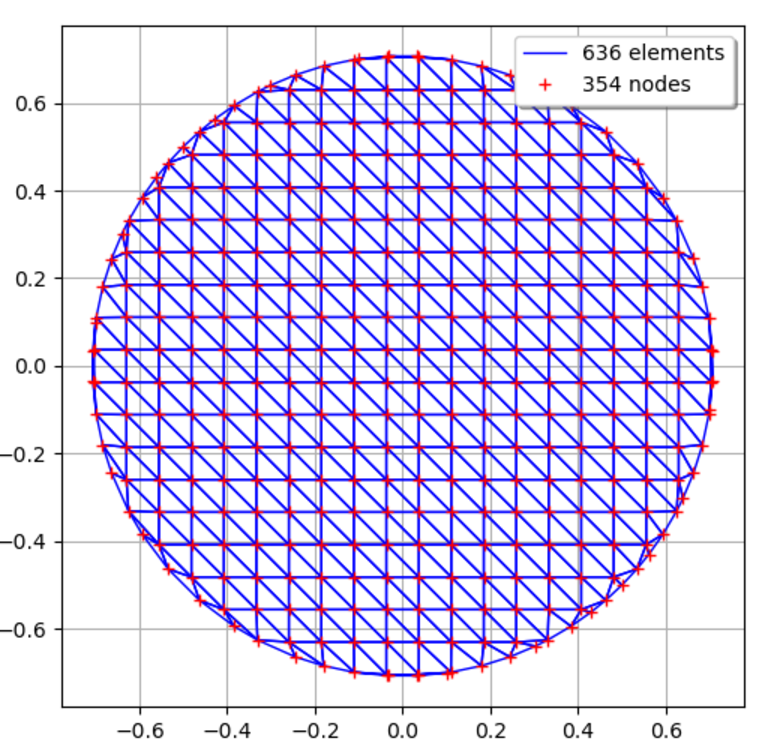
\includegraphics[scale=0.5]{images/meshP1Dim2-750.pdf}
\caption{Maillage d'intéret $M'$ en dimension 2}
\label{maillageInteretDim2}  
\end{center}
\end{figure}


\subsection{Dimension n=3}

On choisit $\bar{D}= [-1,1]^3$ et pour $m \in \mathbb{N}^{*}, \; m > 1$, le maillage $M$ sera caractérisé par des n\oe uds du type
\begin{equation*} \biggl (\biggl(-1 + \frac{2i}{m-1}, -1 + \frac{2j}{m-1}, -1 + \frac{2k}{m-1}\biggr)\biggr)_{(i,j,k) \in \llbracket 0;m-1 \rrbracket^3}  \end{equation*}
et leurs éléments tétraédriques sont décrits de la même façon qu'à la sous-section~\ref{choDim3} du chapitre~\ref{chapCholesky}.
Si on note $h_M$ le maximum des diamètres des éléments triangulaires qui composent le maillage $M$, $h_M = \sqrt{3} \cdot \frac{2}{m-1}$ .\\
Le nombre de n\oe uds $n_M = m^3$ variera entre $10$ et $10000$ et on ne considérera qu'une seule fonction de covariance $C$:
\begin{equation*} C(x,y) = \exp(-\|y-x\|_2^2)  \text{ pour } (x,y) \in (\bar{D})^2 \end{equation*}
~\\
Le maillage $M'$ est défini en deux temps. D'abord on discrétise le domaine $\bar{D}$ par un maillage $BE$ dont on
note $n_{BE}$ le nombre de n\oe uds. Pour \\$m_{BE} \in \mathbb{N}^{*}, \; m_{BE} > 1$, le maillage $BE$ sera caractérisé par des n\oe uds du type
\begin{equation*} \biggl (\biggl(-1 + \frac{2i}{m_{BE}-1}, -1 + \frac{2j}{m_{BE}-1}, -1 + \frac{2k}{m_{BE}-1}\biggr )\biggr)_{(i,j,k) \in \llbracket 0;m_{BE}-1 \rrbracket^3}  \end{equation*}
et leurs éléments tétraédriques sont décrits de la même façon qu'à la sous-section~\ref{choDim3} du chapitre~\ref{chapCholesky}.\\
Le nombre de n\oe uds $n_{BE} = m_{BE}^3$ est fixé à 1000.
On pose ensuite la fonction $f: (x,y,z)  \rightarrow 1 - \sqrt{x^2 + y^2 + z^3}$ et $v=1 - \frac{1}{\sqrt[3]{2}}$.
On obtient alors le maillage d'intérêt $M'$ en parcourant les éléments tétraédriques et en raisonnant de la façon suivante: si tous les sommets $s$
de l'élément vérifient $f(s)> v$ alors on enlève cet élément du maillage, sinon
si un sommet $s$ (mais pas tous) vérifie  $f(s)> v$ alors on modifie la position
du sommet $s$ de façon à ce qu'il vérifie $f(s) = v$.
Le maillage $M'$ ainsi obtenu est un maillage de la boule de centre $0$ et de rayon $v=\frac{1}{\sqrt[3]{2}}$.\\
\phantom{oyez}\\

\begin{figure}[h]
\begin{center}
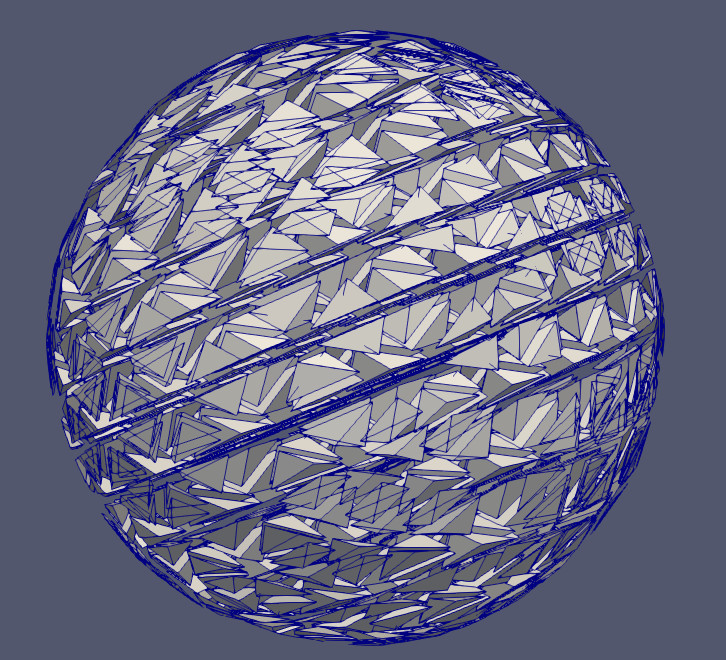
\includegraphics[scale=0.4]{images/meshP1Dim3-750.jpg}
\caption{Maillage d'intéret $M'$ en dimension 3}
\label{maillageInteretDim3}  
\end{center}
\end{figure}

\newpage

\subsection{Benchmarks}

\begin{table}[htbp]
\centering
\begin{tabular}{|>{\centering\arraybackslash}p{1.7cm} |>{\centering\arraybackslash}p{1.5cm} |>{\centering\arraybackslash}p{1.3cm} |>{\centering\arraybackslash}p{1.5cm} |}
\hline
Dimension & Nb de n\oe uds de $M'$ & Nb de n\oe uds de $M$ $n_{M}$ & Temps moyen d'une réalisation (en seconde)  \\
\hline
2 & 354 & 9 & 0.00457s  \\
\hline
2 & 354 & 100 & 0.00558s  \\
\hline
2 & 354 & 961 & 0.11667s  \\
\hline
2 & 354 & 10000 & 146.70s  \\
\hline
\hline
3 & 474 & 8 & 0.01782s  \\
\hline
3 & 474 & 64 & 0.02263s  \\
\hline
3 & 474 & 729 & 0.09118s  \\
\hline
3 & 474 & 9261 & 117.63s  \\
\hline
\end{tabular}
\end{table}

\begin{table}[htbp]
\centering
\begin{tabular}{|>{\centering\arraybackslash}p{1.7cm} |>{\centering\arraybackslash}p{1.5cm} |>{\centering\arraybackslash}p{1.3cm} |>{\centering\arraybackslash}p{1.5cm} |>{\centering\arraybackslash}p{1.5cm} |>{\centering\arraybackslash}p{1.2cm}|}
\hline
Dimension & Nb de n\oe uds de $M'$ & Nb de n\oe uds de $M$ $n_{M}$ & $h_M$ & Nb de réalisations & erreur $L^2$ \\
\hline
2 & 354 & 16 & 0.94280 & 250 & 0.09704   \\
\hline
2 & 354 & 16 & 0.94280 & 1000 & 0.13483   \\
\hline
2 & 354 & 16 & 0.94280 & 4000 & 0.11302   \\
\hline
2 & 354 & 16 & 0.94280 & 10000 & 0.11756   \\
\hline
\hline
2 & 354 & 121 & 0.28284 & 250 & 0.08694   \\
\hline
2 & 354 & 121 & 0.28284 & 1000 & 0.02646   \\
\hline
2 & 354 & 121 & 0.28284 & 4000 & 0.01703   \\
\hline
2 & 354 & 121 & 0.28284 & 10000 & 0.01040   \\
\hline
\hline
2 & 354 & 529 & 0.12856 & 250 & 0.16377   \\
\hline
2 & 354 & 529 & 0.12856 & 1000 & 0.01925   \\
\hline
2 & 354 & 529 & 0.12856 & 4000 & 0.01875   \\
\hline
2 & 354 & 529 & 0.12856 & 10000 & 0.00689   \\
\hline
\hline
2 & 354 & 1024 & 0.09123 & 250 & 0.04241   \\
\hline
2 & 354 & 1024 & 0.09123 & 1000 & 0.01526   \\
\hline
2 & 354 & 1024 & 0.09123 & 4000 & 0.04384   \\
\hline
2 & 354 & 1024 & 0.09123 & 10000 & 0.01988   \\
\hline
\hline
3 & 474 & 27 & 1.7320 & 250 & 0.43154 \\ 
\hline
3 & 474 & 27 & 1.7320 & 1000 & 0.43918 \\ 
\hline
3 & 474 & 27 & 1.7320 & 4000 & 0.45128 \\ 
\hline
3 & 474 & 27 & 1.7320 & 10000 & 0.45764 \\ 
\hline
\hline
3 & 474 & 125 & 0.86602 & 250 & 0.17489 \\ 
\hline
3 & 474 & 125 & 0.86602 & 1000 & 0.18455 \\ 
\hline
3 & 474 & 125 & 0.86602 & 4000 & 0.17802 \\ 
\hline
3 & 474 & 125 & 0.86602 & 10000 & 0.15349 \\
\hline
\hline
3 & 474 & 512 & 0.49487 & 250 & 0.14222 \\ 
\hline
3 & 474 & 512 & 0.49487 & 1000 & 0.07678 \\ 
\hline
3 & 474 & 512 & 0.49487 & 4000 & 0.07379 \\ 
\hline
3 & 474 & 512 & 0.49487 & 10000 & 0.06428 \\ 
\hline
\hline
3 & 474 & 1000 & 0.38490 & 250 & 0.11127 \\ 
\hline
3 & 474 & 1000 & 0.38490 & 1000 &  0.05500\\ 
\hline
3 & 474 & 1000 & 0.38490 & 4000 & 0.03705 \\ 
\hline
3 & 474 & 1000 & 0.38490 & 10000 & 0.02903 \\ 
\hline
\end{tabular}
\end{table}


\newpage

\begin{figure}[h]
\begin{center}
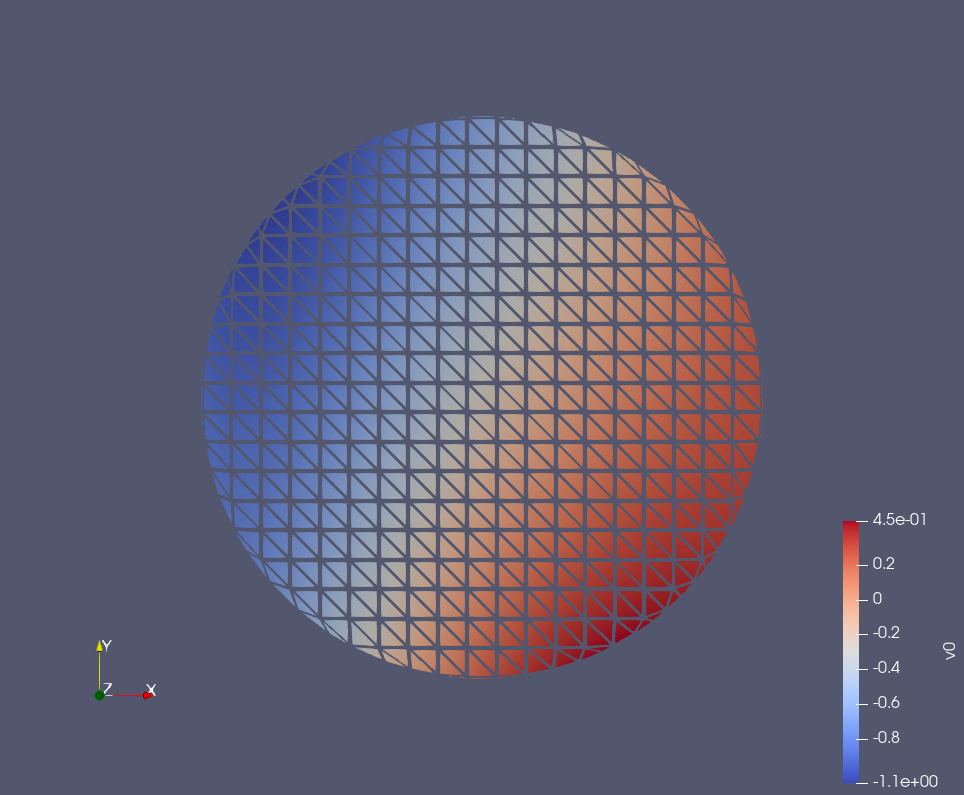
\includegraphics[scale=0.3]{images/meshP1Dim2-750-961.png}
\caption{Réalisation sur $M'$ en dimension 2 où $n_{M} = 961$ }
\label{ReaDim2-961}  
\end{center}
\end{figure}


\phantom{oyez}\\

\uppercase{à} des fins de comparaison, on rajoute ci-dessous un benchmark où on applique directement la méthode de Cholesky sur le maillage d'intérêt $M'$. On ne considère donc plus
le maillage $M$.\\
\phantom{oyez}

\begin{table}[htbp]
\centering
\begin{tabular}{|c |c |c |c |}
\hline
Dimension & Nb de n\oe uds de $M'$ & Nb de réalisations  & erreur $L^2$ \\
\hline
2 & 354 & 250 & 0.04956   \\
\hline
2 & 354 & 1000 & 0.01539   \\
\hline
2 & 354 & 4000 & 0.01319    \\
\hline
2 & 354 & 10000 & 0.01148   \\
\hline
\hline
3 & 474 & 250 & 0.17656 \\ 
\hline
3 & 474 & 1000 & 0.08154 \\ 
\hline
3 & 474 & 4000 & 0.03933 \\ 
\hline
3 & 474 & 10000 & 0.01620 \\ 
\hline
\end{tabular}
\end{table}



%\newpage

%\begin{figure}[h]
%\centering
%\begin{tikzpicture}
%\begin{axis} [ybar,
%height=3.2cm,
%width=10cm,
%axis x line=center,
%axis y line=center,
%xlabel style={below right},
%ylabel style={above left},
%xmin=5.0,
%xmax=9.5,
%xlabel = {$\ln(N_{rea})$},
%ylabel = {erreur $L^2$},
%ymin=0.0,
%ymax=0.25
%]
%\addplot coordinates {
%    (5.52146,0.17656) 
%    (6.90775,0.08154) 
%    (8.29404,0.03933) 
%    (9.21034,0.01620)
%};
%\end{axis}
%\end{tikzpicture}
%\caption{$n=2$, $n_M = 354$}
%\end{figure}









